\lab{Filtering and Convolution}{Filtering and Convolution}
\objective{The Fourier transform reveals things about an audio signal that are not immediately apparent from the soundwave. In this lab we learn to filter noise out of a signal using the discrete Fourier transform, and explore the effect of convolution on sound files.}

% TODO:
%       - Address stereo vs. mono signals, especially for the convolution.

\section*{Cleaning up a Noisy Signal}

Listen to \texttt{Noisysignal1.wav}.
This is a mono recording of a (probably familiar) voice with some annoying noise over it.
The plot of the soundwave isn't very descriptive; in fact, it looks like static.
See Figure \ref{fig:noisysignal}.

\begin{figure}
\centering
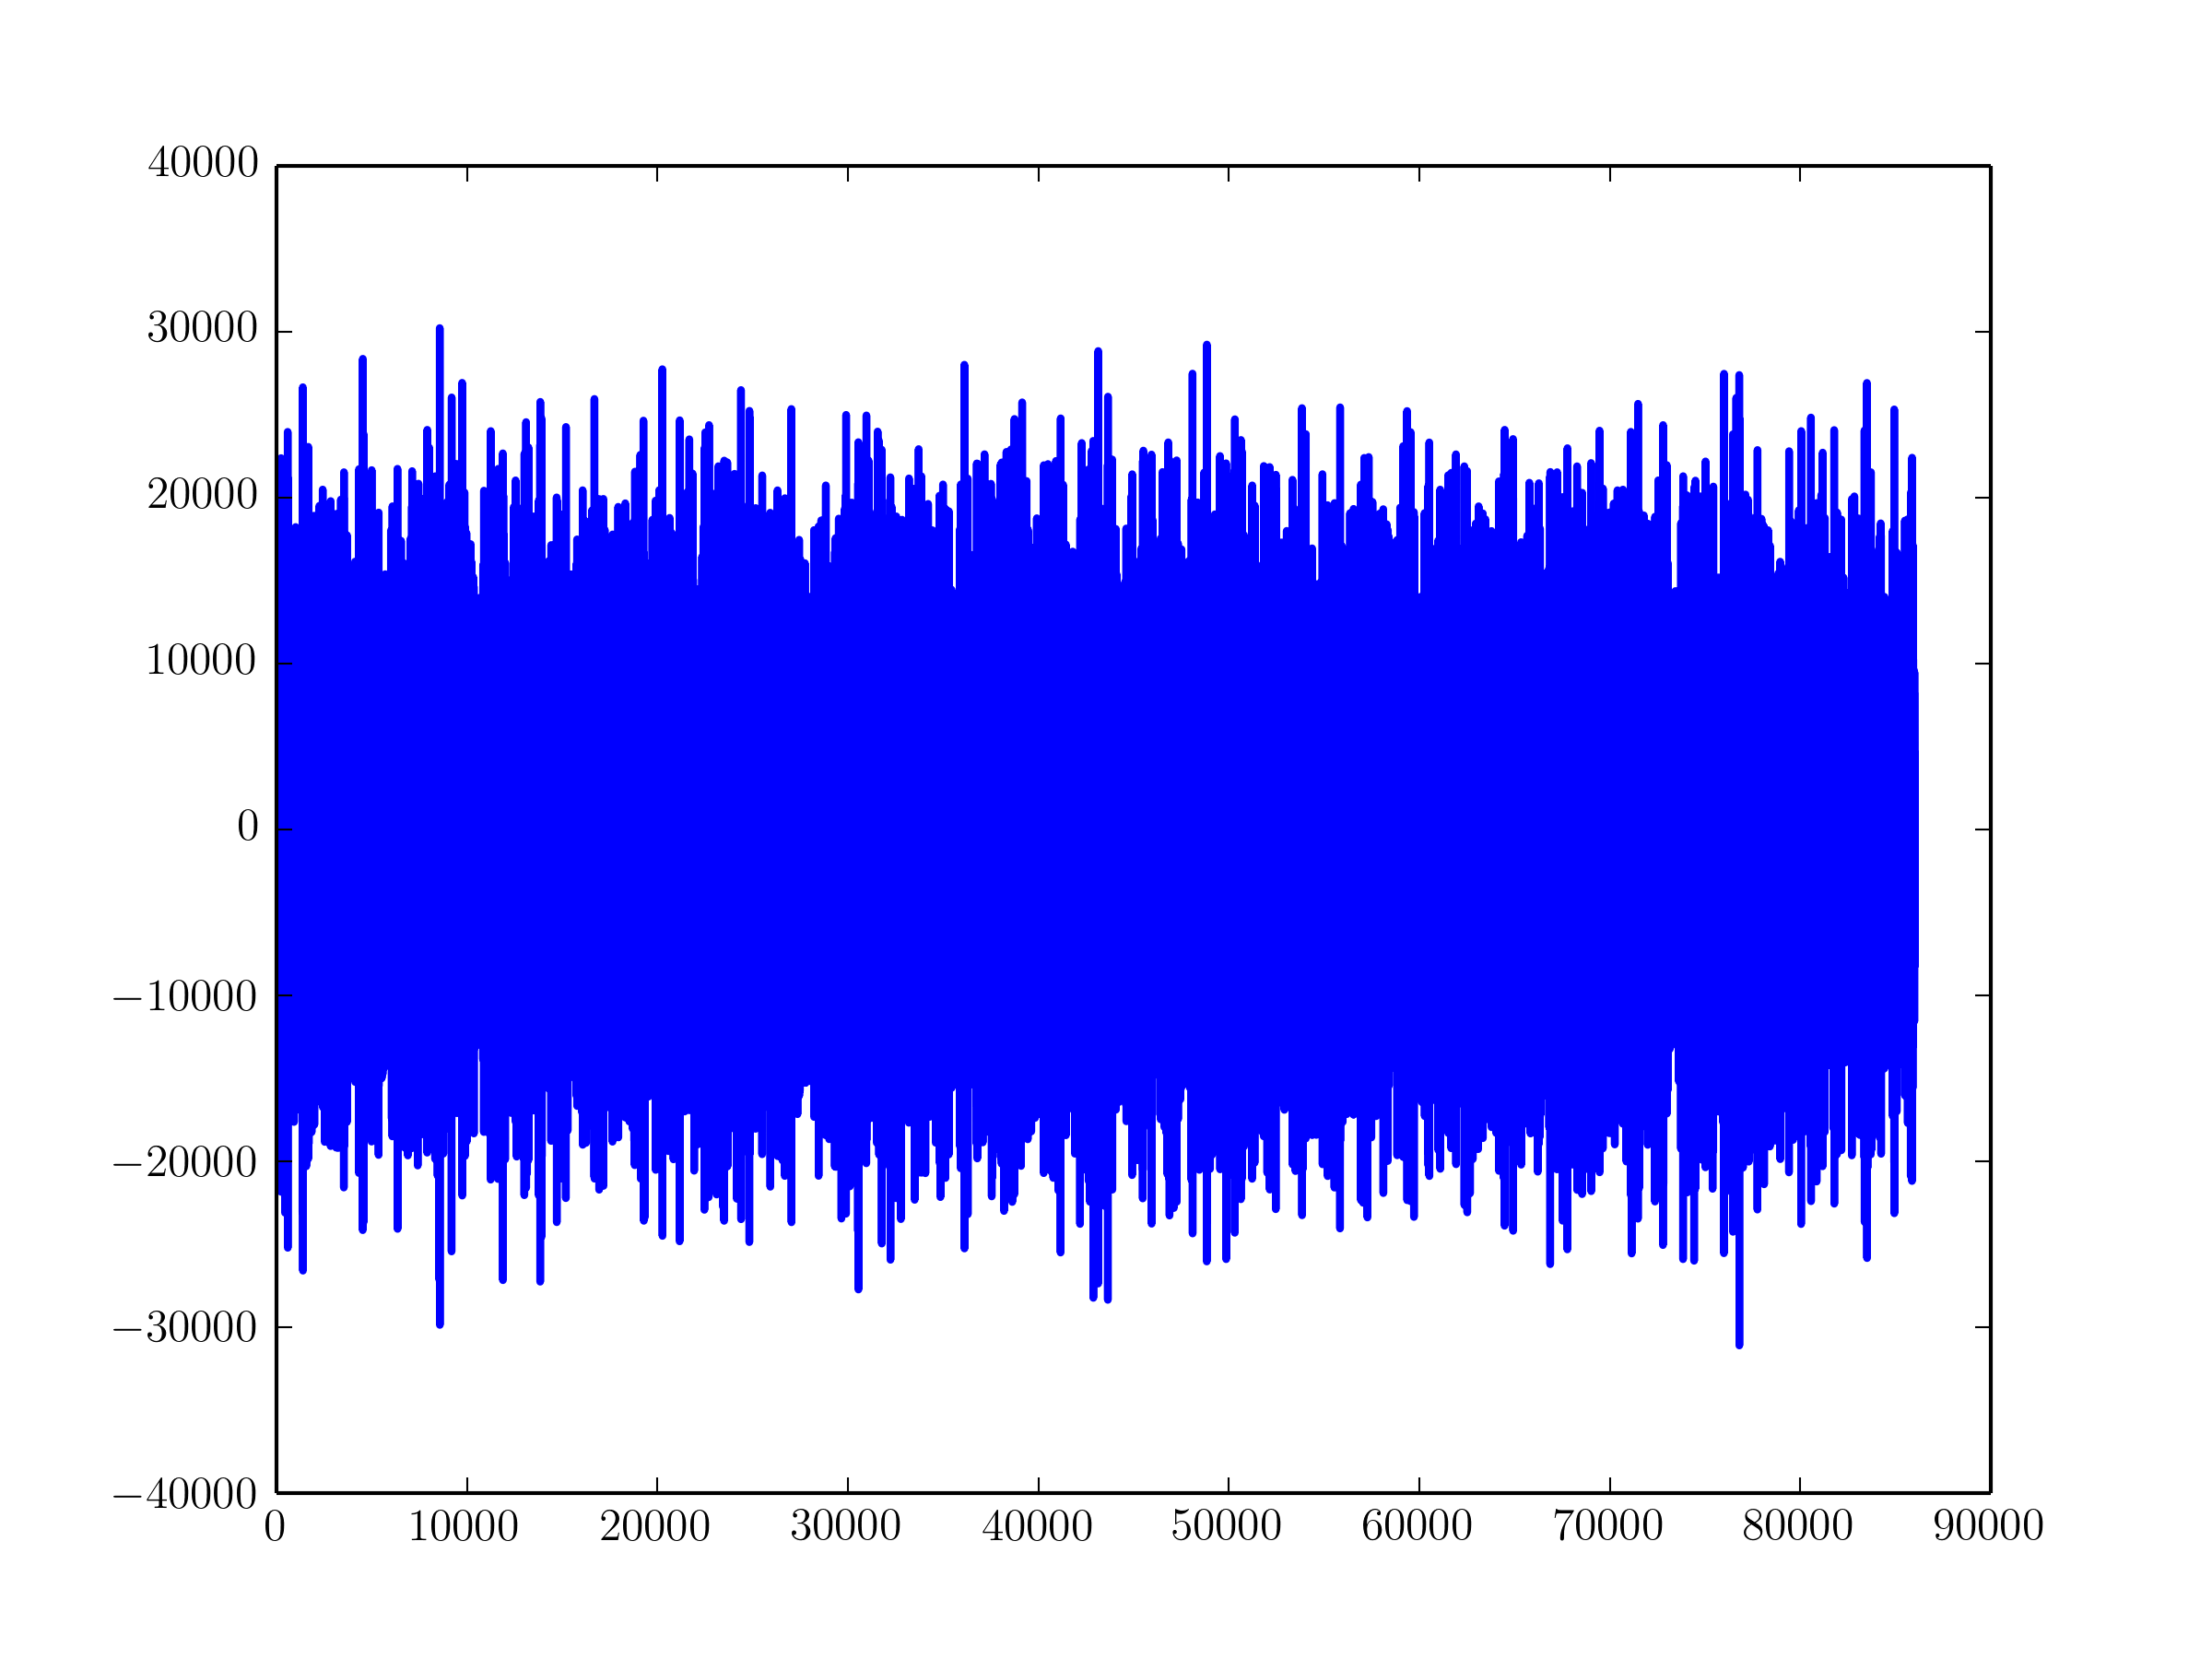
\includegraphics[width=\textwidth]{figures/noisy}
\caption{The plot of \texttt{Noisysignal1.wav}.}
\label{fig:noisysignal}
\end{figure}

However, if we take the Fourier transform of the signal, we see that the static in Figure \ref{fig:noisysignal} is the result of some concentrated high frequency noise.
(In this case, artificially added).
See Figure \ref{fig:noisyspec}.

\begin{figure}
\centering
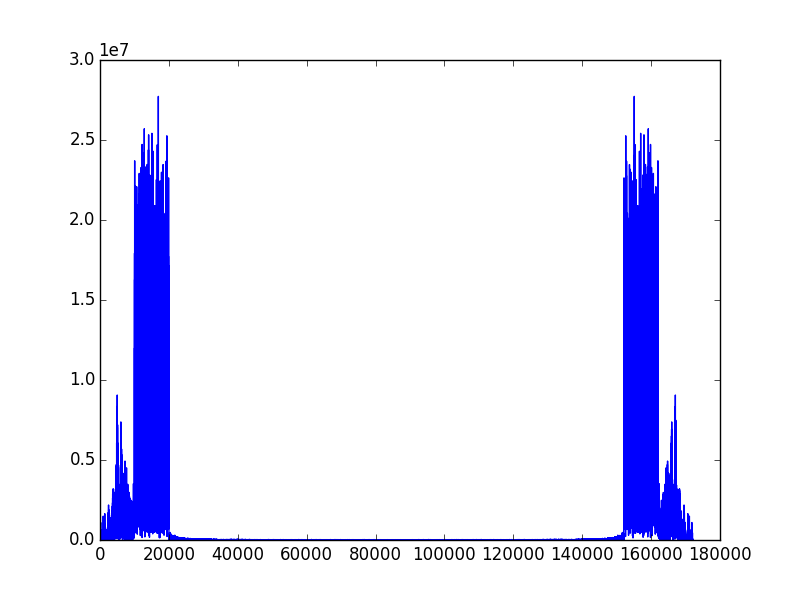
\includegraphics[width=\textwidth]{figures/noisyspec}
\caption{Spectrum of \li{Noisysignal1.wav}}
\label{fig:noisyspec}
\end{figure}

The noise can be removed by setting the coefficients of the high frequencies to zero.
Since the discrete Fourier transform is symmetric, if we set coeffecient $j$ to $0$, then we must set coefficient $N - j$ to $0$ as well, where $N$ is the number of coefficients.
Then we calculate the inverse Fourier transform to get a new, clean signal.

\begin{lstlisting}
>>> rate,data = wavfile.read('Noisysignal1.wav')

# Calculate the Fourier transform
>>> fsig = sp.fft(data, axis = 0)

# Coefficients 10000 to 20000 were chosen by inspecting the
# plot of the Fourier transform.
>>> for j in xrange(10000, 20000):
...     # Set the chosen coefficients to 0
...     fsig[j] = 0
...     fsig[-j] = 0

# Calculate the inverse Fourier transform, cast it as real,
# and scale it to be compatible with the wavfile format.
>>> newsig = sp.ifft(fsig)
>>> newsig = sp.real(newsig)
>>> newsig = sp.int16(newsig / sp.absolute(newsig).max() * 32767)
\end{lstlisting}

Now we can save the resulting cleaned-up signal \texttt{newsig} to a \li{.wav} file.
The plot of the wave now reveals individual syllables as they are spoken.
See Figure \ref{fig:cleansignal}.

\begin{figure}
\centering
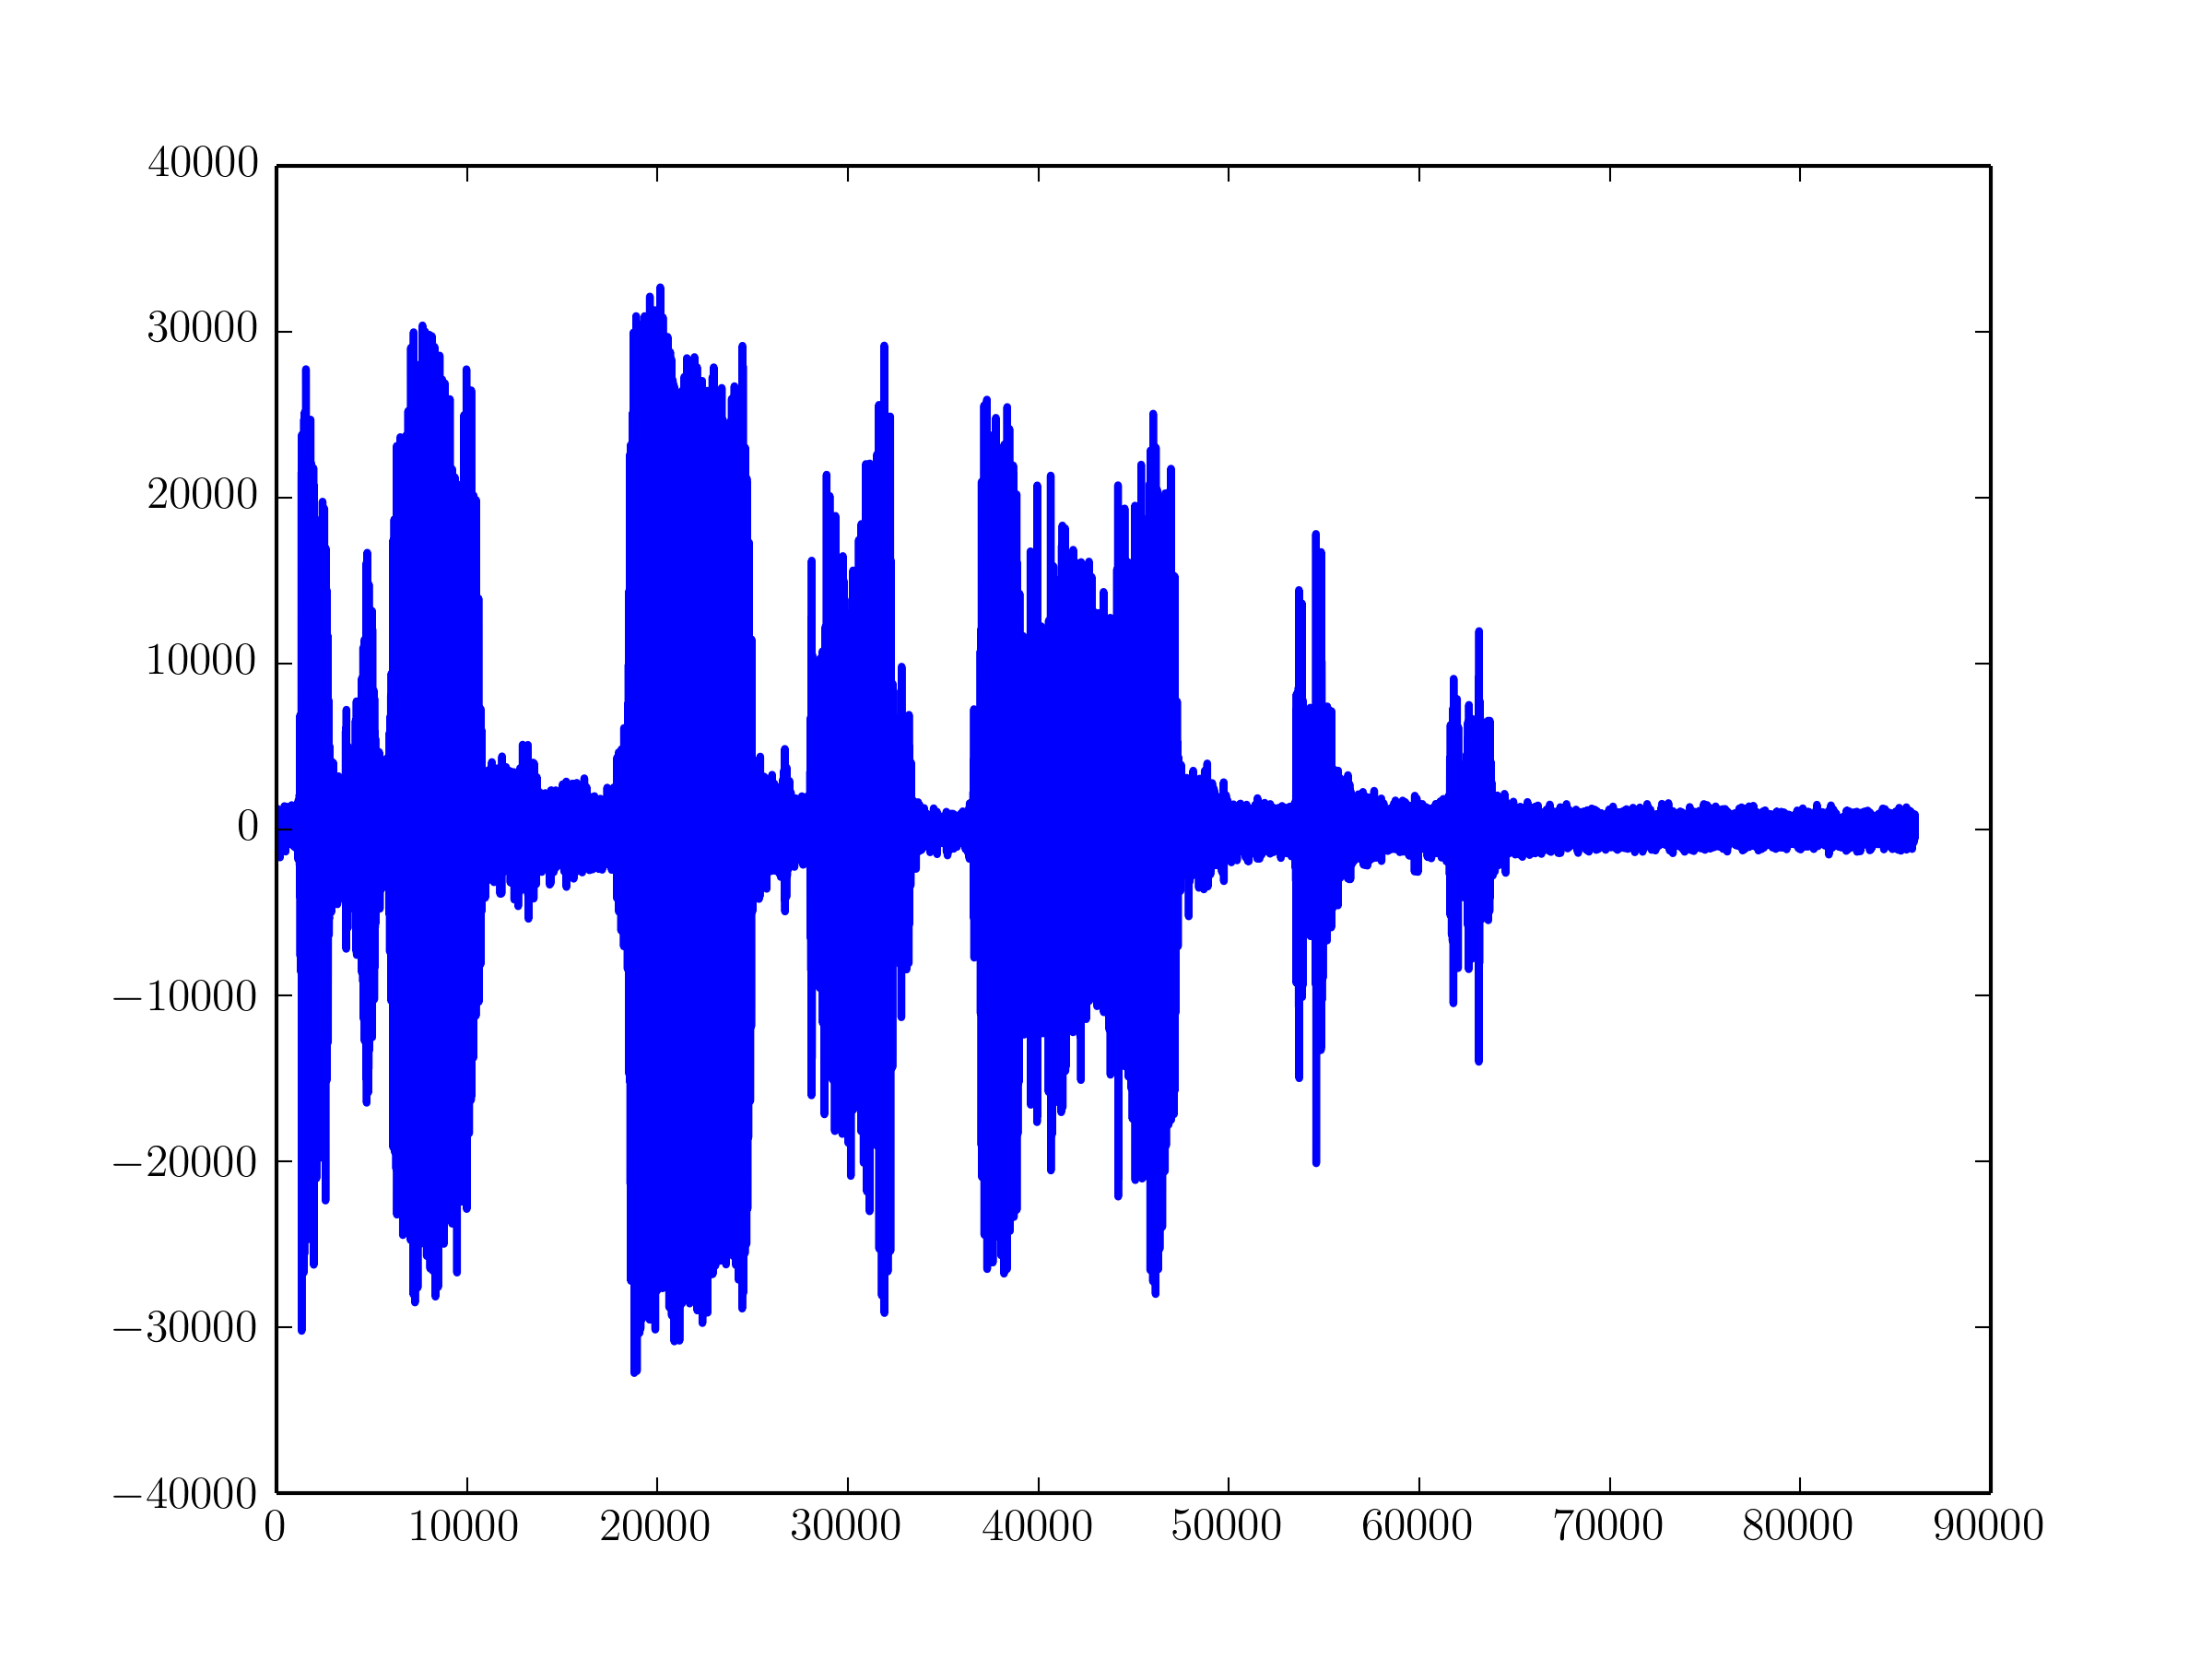
\includegraphics[width=\textwidth]{figures/Cleanedsignal}
\caption{The plot of \texttt{Noisysignal1.wav} after being cleaned.}
\label{fig:cleansignal}
\end{figure}

% Problem 1: Clean up a noisy signal (The only thing we have to fear...)
\begin{problem}
Listen to \texttt{Noisysignal2.wav}.
You will probably just hear noise.
Inspect the discrete Fourier transform to see where there is noise.
Remove the noise using the technique described above in order to make the cleaned-up signal audible.
What does the voice say?
Who is the speaker?
(If you don't know the answer to this last question, try a quick Google search.)
\end{problem}

The DFT is commonly used in sound filtering, though identifying the particular frequencies to zero out can be difficult.

\section*{Filtering and Convolution}

The DFT is useful for more than filtering noise out of a signal.
Suppose we have a recording of musical piece played in a small carpeted room with essentially no acoustics (little or no echo), and suppose we would like to apply an effect to make it sound as if the piece were played in a large concert hall or some other room.
The DFT makes this possible when used together with the idea of \emph{convolution}.

When a balloon is popped in large room, although the sound of the actual pop only lasts a few milliseconds, the sound echoes about the room for up to several seconds.
This echoing sound is called an \emph{impulse response} of the room, and is a way of approximating the acoustics of a room.

So first, we need a recording of how the room responds to a short pulse of sound.
Effective ways of producing a loud sound approximating a pulse include firing a (blank) gunshot, popping a balloon, or, if neither of those are available, clapping the hands one time.

Recall that we model sound with discrete samples of a soundwave in rapid succession.
When these sounds are played back, the ear percieves them as a continuous soundwave.
In other words, sound playback is a series of pulses of varying intensities, similar to the pulse in an impulse response.
If we ``mix'' the individual sounds of an instrument in a carpeted room with the impulse response from a concert hall, then the new soundwave will sound as if the instrument is being played in the concert hall.

Since audio needs to be samples frequently (44100 samples per second is standard) to create smooth playback, a recording of a song can be millions of samples.
Each of these samples needs to be combined with the impulse response, which may be several seconds long.
This may be starting to seem computationally infeasible or at least very difficult.
The key is to recognize that this process can be described as a convolution: namely, the final sound is simply the convolution of the our original sound with the impulse response.
We can calculate convolutions quickly using the convolution theorem:

\[\mathcal{F}(f \ast g) = \mathcal{F}(f)\cdot\mathcal{F}(g)\]

where $\mathcal{F}$ is the Fourier Transform, $\ast$ is convolution, and $\cdot$ is component-wise multiplication.
Thus we calculate the convolution of two arrays by simply taking the Fourier transform of each, multiplying them pointwise, and then taking the inverse transform.

% Problem 2 (Optional): Get a good ballon pop to convolve stuff with.
\begin{problem}
(Optional)\footnote{If the instructor does not require this problem then students may use the provided \texttt{balloon.wav} file which contains the sound of a balloon pop in a large room.} Find a large room or area with good acoustics, and record (an approximation to) its impulse response using a balloon pop.
To record the sound, you will want to use at least a decent microphone.
You may want to record it using the program Audacity\footnote{Audacity is free sound manipulation software and may be downloaded at http://audacity.sourceforge.net} and a laptop.
If you use a unidirectional microphone, be sure the microphone is pointing at the balloon when you pop it, so that the direct sound from the pop is picked up.
(If you don't, the result will still be okay.
However, after the convolution it will probably sound somewhat distant, as if we were standing somewhere where we couldn't hear the music directly.)
If you've chosen a good room, the response should be audible for at least a full second.

Include a plot of both the waveform and spectrum of the impulse response you recorded.
\end{problem}

% Problem 3: Convolve the balloon pop with Chopin.
\begin{problem}\label{convolution_problem}
Download and listen to the file \texttt{chopin.wav}.
You will hear a piano being played in a dead room with little or no acoustics.
Using the Convolution Theorem, take the convolution of this signal with the impulse response recorded in the previous problem.
The convolution given in the theorem is \emph{circular}, meaning that sounds at the end of the signal will tend to mix with sounds at the beginning of the signal.
To avoid this effect, add several seconds of silence to the end of \li{chopin.wav} by appending zeroes to the end of the signal.
Also, keep in mind that the Convolution Theorem requires both signals to have the same length; therefore you will need to pad the smaller of your two signals (namely, the impulse response signal) with zeros in order to make it the same size as the other signal.
These zeros should be added to the middles of signals, as we need to maintain its symmetric structure.
Describe the resulting sound.

To summarize:
\begin{enumerate}

\item Read in \texttt{chopin.wav} and the impulse response with \li{wavfile},
\item Add several seconds of silence to the signal from \texttt{chopin.wav},
\item Insert zeros into the middle of the impulse response transform so that it is the same length as,
\item Calculate the convolution of the signals,
\item And finally, calculate the inverse Fourier transform.
\end{enumerate}

\end{problem}

In some instances, a circular convolution is actually desirable.
For instance, an interesting effect is achieved by taking the circular convolution of a long segment of white noise with some other (shorter) sound.
We can create white noise using SciPy's \li{random} module:
\begin{lstlisting}
# Create 10 seconds of mono white noise.
samplerate = 22050
noise = sp.int16(sp.random.randint(-32767, 32767, samplerate * 10))
\end{lstlisting}

% Problem 4: White noise.
\begin{problem}
Create white noise and listen to the resulting sound (\textbf{CAUTION:} Turn your volume way down. It may be very very loud).
This kind of noise is called ``white" because it contains all frequencies with the same strength, or rather, with the same expected strength (since the amplitude of a specific frequency is a matter of chance).
In order to see this, plot the spectrum of the noise.
\end{problem}

Now can take the circular convolution of this noise with some other sound.
For instance, let's use \texttt{tada.wav}.
The result is in \texttt{tada-conv.wav}.
We notice that the original short sound has been sustained to an indefinite length.
The result is not a set of static tones, but rather a rich sound which preserves not only the tones, but the texture, of the original sound; you can hear different tones fluctuating randomly in amplitude over time.
If you were to play this \texttt{tada-conv.wav} on repeat, you would find that, because we used a circular convolution, the sound loops seamlessly from the end back to the beginning; however, most sound players are not capable of doing this properly, so you will probably hear a break in the sound. To demonstrate the ``seamlessness", we can paste together three copies of the sound consecutively:

\begin{lstlisting}
rate, sig = wavfile.read('tada-conv.wav')
sig = sp.append(sig, sig)
sig = sp.append(sig, sig)
\end{lstlisting}

Listen to the resulting sound, and notice that we are not able to identify where the sound loops back to the beginning, because there is no break or click.

% Useless old problem.
\begin{comment}
\begin{problem}
Record yourself singing a few notes (or, feel free to produce some other sound another way).
Take the circular convolution of white noise with this recording.
Now do it again using stereo white noise.
This is just like the mono white noise problem, but make the SciPy array in two dimensions.
It's no problem that your original recording will probably be mono; just make the left and right channels duplicate in the recording (but: be sure to use different left and right channels for the white noise).
Can you hear any difference between the mono and stereo versions of the result?
\end{problem}

Feel free to play around with this. The file \texttt{guitar-conv.mp3} is a collage of sounds created using this technique (mostly using guitar samples). You could probably think of other lots of other things you can do with this.
\end{comment}

